\Exercise Troba els punts estacionaris, i el seu tipus, de la funció $f(x)=2x^3-3x^2-36x+2$
\label{ex:puntsestacionaris1}
\Answer


En trobem primer la derivada i la igualem a zero per tal de trobar els punts estacionaris:

\[f'(x)=6x^2-6x-36=6(x^2-x-6)=0\]

\[x=\frac{1\pm\sqrt{1^2-4\cdot1\cdot(-6)}}{2}=\left\{\begin{array}{c}3\\-2\end{array}\right.\]

Un cop trobats, per saber de quin tipus són fem la segona derivada i els hi substituïm:
\[f''(x)=6(2x-1)\]
\[f''(x=3)=30>0\]
\[f''(x=-2)=-30<0\]

Per tant, la funció té un màxim a $x=-2$ i un mínim a $x=3$, com es pot veure al gràfic de la Figura \ref{fig:puntsestacionaris1}.

\begin{center}
\begin{minipage}{8cm}
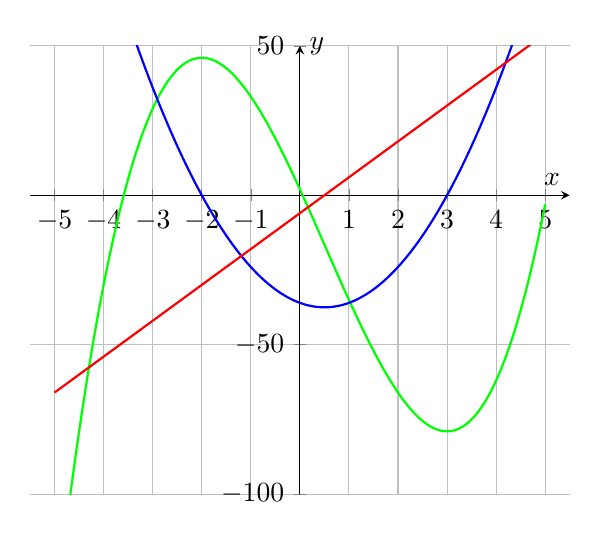
\begin{tikzpicture}[>=latex]
  \begin{axis}[%axis equal,
    axis lines=middle, 
    xmin=-5, xmax=5,
    ymin=-100, ymax=50,
    xtick={-5,...,5},
    ytick={-100,-50,0,50},
    grid=major,
    samples=222,
    xlabel={$x$},
    xlabel style = {anchor=south east},
    ylabel={$y$},
    ylabel style = {anchor=west},
    enlarge x limits={abs=0.5},
  ]
  \addplot[draw=green, thick, mark=none,domain=-5:5]{2*x^3-3*x^2-36*x+2}; 
  \addplot[draw=blue, thick, mark=none,domain=-5:5]{6*x^2-6*x-36};    
  \addplot[draw=red, thick, mark=none,domain=-5:5]{12*x-6};

  \end{axis}
  \end{tikzpicture}
  \captionof{figure}{$f(x)$ (verd), $f'(x)$ (blau) i $f''(x)$ (vermell) de l'Exercici \ref{ex:puntsestacionaris1}.}
  \label{fig:puntsestacionaris1}
\end{minipage} 
\end{center}

Aquest codi permet resoldre l'exercici a \texttt{MATLAB}:
\begin{lstlisting}[style=Matlab-editor]
  % resolució exercici
  syms x
  f=2*x^3-3*x^2-36*x+2
  fplot(f)
  f1=diff(f)
  f2=diff(f1)
  solve(f1==0)
  \end{lstlisting}


\blacksquare 